\problemname{Light show}
\noindent
Your friend is designing a light show for the closing ceremony of this year's Programming Olympiad finals.
The hall where the ceremony is held can be viewed as a grid with $R$ rows and $C$ columns.
Different lamps are mounted along the four sides, which can shine in one of three different colors: red, blue, or green.
During the ceremony, the idea is that the lamps will shift in different patterns.

\begin{figure}[h]
    \centering
    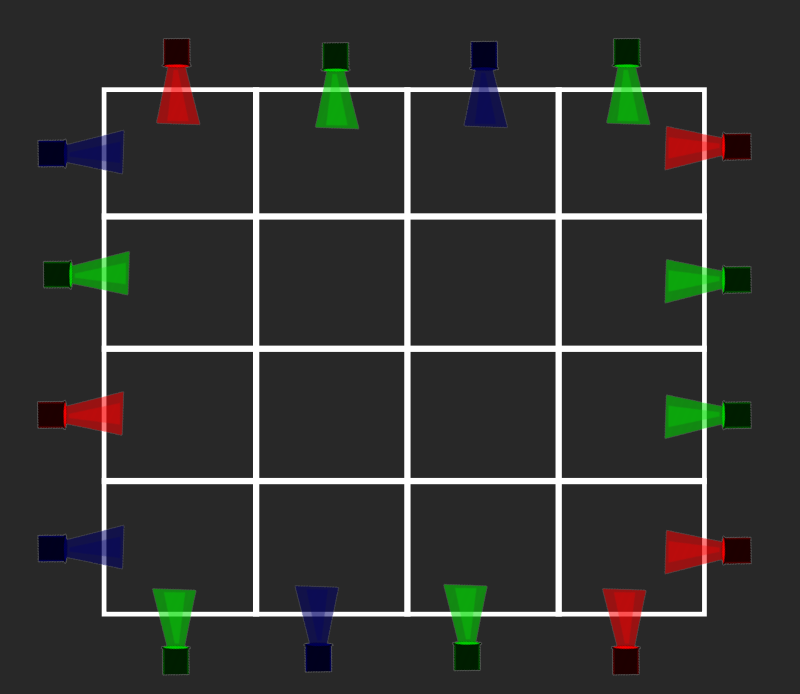
\includegraphics[width=0.6\textwidth]{affischbild}
    \caption{An example of a lamp color configuration, where $R = C = 4$. The example corresponds to the only test case in test group 1.}
\end{figure}

A lamp illuminates all the squares along the same column or row where it is mounted.
If a certain square is illuminated by at least one lamp of each color, the light in the square will be perceived as an unpleasant glaring white.
Your friend has already designed a draft of the light show and now wonders if some of the chosen light configurations cause too many squares to become white.
To determine whether a configuration is okay or not, you have been tasked with writing a program that reads the color of all the lamps and calculates the number of squares that will shine white.

\section*{Input}
The first line contains two integers $R$ ($1 \le R \le 10^6$) and $C$ ($1 \le C \le 10^6$), the number of rows and columns in the grid-shaped hall.

The next four lines each contain a text string describing the colors of all the lamps.
The first line describes the $C$ lamps at the top of the grid shining downwards in order from left to right,
the second line describes the $R$ lamps to the right of the grid shining to the left in order from top to bottom,
the third line describes the $C$ lamps below the grid shining upwards in order from left to right,
the fourth line describes the $R$ lamps to the left of the grid shining to the right in order from top to bottom.

The color of a lamp is described using the characters \texttt{RGB} depending on whether the lamp shines red, green, or blue.

\section*{Output}
Print a single integer -- the number of squares in the hall that shine white.
\textbf{Note: the answer does not necessarily fit in a 32-bit integer.}

\section*{Scoring}
Your solution will be tested on a set of test groups, each worth a number of points. Each test group contains
a set of test cases. To get the points for a test group you need to solve all test cases in the test group.

\noindent
\begin{tabular}{| l | l | p{12cm} |}
  \hline
  \textbf{Group} & \textbf{Points} & \textbf{Constraints} \\ \hline
  $1$    & $20$        &  The group consists of a single test case, the one on our poster (\url{https://www.progolymp.se/2022/affisch.pdf}). \\ \hline 
  $2$    & $15$        &  All lamps on the same side have the same color. \\ \hline
  $3$    & $25$        &  $R,C \le 1000$ \\ \hline 
  $4$    & $25$        &  All lamps to the right or left of the grid shine red, and all lamps above and below the grid shine green or blue. \\ \hline
  $5$    & $15$        &  No additional constraints. \\ \hline
\end{tabular}

\section*{Explanation of Example Cases}
In the first case, all squares in the only row are illuminated by red from both left and right.
The first square is illuminated by green from both above and below, the second and fourth squares by both green and blue, while the third is only illuminated by blue.
Thus, two of the squares are illuminated by all three colors and become white.

In the third example, blue light is completely absent.
Therefore, no squares can be white.
